\documentclass[10pt,twocolumn,letterpaper]{article}

\usepackage{cvpr}
\usepackage{times}
\usepackage{epsfig}
\usepackage{graphicx}
\usepackage{amsmath}
\usepackage{amssymb}
\usepackage{listings}
\usepackage{xcolor}
\usepackage[table,xcdraw]{xcolor}
\usepackage{caption}
\usepackage{makecell}
\usepackage[T1]{fontenc}
\usepackage{placeins}
\usepackage{booktabs}
\usepackage{algorithm}
\usepackage{algpseudocode}

\definecolor{lightergray}{rgb}{0.9,0.9,0.9}
\renewcommand{\arraystretch}{1.15}
\captionsetup[table]{skip=5pt}

\lstset{
    language=Python,
    basicstyle=\ttfamily\small,
    keywordstyle=\color{blue},
    stringstyle=\color{red},
    commentstyle=\color{green},
    showstringspaces=false,
    frame=single,
    breaklines=true
}
% Include other packages here, before hyperref.

% If you comment hyperref and then uncomment it, you should delete
% egpaper.aux before re-running latex.  (Or just hit 'q' on the first latex
% run, let it finish, and you should be clear).
\usepackage[breaklinks=true,bookmarks=false]{hyperref}

\cvprfinalcopy % *** Uncomment this line for the final submission

\def\cvprPaperID{****} % *** Enter the CVPR Paper ID here
\def\httilde{\mbox{\tt\raisebox{-.5ex}{\symbol{126}}}}

% Pages are numbered in submission mode, and unnumbered in camera-ready
%\ifcvprfinal\pagestyle{empty}\fi
\setcounter{page}{1}
\begin{document}

%%%%%%%%% TITLE
\title{Can Parrot Be Implemented on Low-End, Cost-Effective Devices for CAN Bus Security?}

\author{
Marco Bernardi \\
{\tt\small marco.bernardi.11@studenti.unipd.it}
}

\maketitle
%\thispagestyle{empty}

%%%%%%%%% ABSTRACT
\begin{abstract}This research aim to reproduce the results of the
    paper " Parrot, a software-only anti-spoofing defense
    system for the CAN bus"~\cite{dagan2016parrot}
\end{abstract}

%%%%%%%%% BODY TEXT
\section{Introduction}
The Controller Area Network (CAN) bus is a widely adopted communication protocol in the automotive industry, valued for its simplicity and efficiency. 
However, as a broadcast bus, it transmits messages to all nodes, making it susceptible to spoofing attacks. 
In such attacks, an adversary injects messages that impersonate legitimate nodes, potentially disrupting system functionality.

This paper implements Parrot, a software-only anti-spoofing defense system for the CAN bus. 
Parrot detects spoofing attacks by analyzing message timing on the bus and mitigates them by forcing the attacker into a bus-off state. 
This approach enhances security without requiring hardware modifications, offering a cost-effective and practical solution for automotive cybersecurity.

\section{Parrot System}
As the title suggests, Parrot is a software-only solution, meaning it does not require any hardware modifications to the CAN bus. 
Its functionality is summarized in Algorithm~\ref{alg:parrot}.
\begin{algorithm}
    \caption{Parrot Algorithm}
    \label{alg:parrot}
    \begin{algorithmic}[1]
        \Procedure{Main}{}
        \State InitializeDefenseSystem()
        \While{parrotOnGuard}
        \If{suspectFound}
        \State \# Identified a spoofed message with my ID
        \State \Call{Engage}{spoofedID}
        \EndIf
        \EndWhile
        \EndProcedure

        \Procedure{Engage}{SPOOFEDID}
        \While{suspectFound \textbf{and not} collisionDetected}
        \State \Call{TransmitNDMessages}{ND}
        \EndWhile
        \EndProcedure

        \Procedure{TransmitNDMessages}{ND}
        \State bound $\gets$ ND
        \For{$i \gets 0$ \textbf{to} $bound - 1$}
        \State transmitDmessage()
        \If{collisionDetected}
        \State collisionDetected $\gets$ \textbf{False}
        \State suspectFound $\gets$ \textbf{False}
        \State \# Transmit exactly 15 more Dmessages
        \State bound $\gets i + 16$
        \EndIf
        \EndFor
        \EndProcedure
    \end{algorithmic}
\end{algorithm}

\section{System Setup}
\subsection{Hardware}
For the replication of the Parrot system, the authors utilized two Raspberry Pi 3 Model B+ devices, running Raspbian OS, configured as the attacker and target Electronic Control Units (ECUs). 
These Raspberry Pi units were connected to the CAN bus using CAN bus shields equipped with the MCP2515 CAN controller, a widely used, cost-effective solution for interfacing with CAN networks, making it an ideal choice for both research and practical applications.
To debug and validate the system's behavior, an oscilloscope was employed to monitor the CAN bus signals in real-time. 
This allowed for precise observation of signal timing, detection of potential collisions, and verification of message integrity on the bus. 
The use of an oscilloscope was critical in ensuring that the Parrot system's functionality adhered to the expected behavior under various conditions, including spoofed message attacks and defense countermeasures.

\subsection{Software}
The mocked ECU software (and so on the Parrot system) is implemented in Python using the python-can library.
All the code is available on the GitHub repository of the authors~\cite{parrot_github}.

\section{Experiment}

In this experiment, the attacker was set up to send a spoofed message with the ID of the target ECU and a random payload. The actual payload data is not of concern for this experiment; what matters is that the payload is not all zeroes (0x00), as the defense mechanism will use messages with a payload of 0x00 as a countermeasure against the attacker.

\subsection{CAN Arbitration Mechanism}

The CAN protocol operates with a bitwise arbitration mechanism, where messages are transmitted bit by bit, and each ECU can "listen" to the bus while it is transmitting. If both the attacker and the defender (target ECU) attempt to transmit the same message at the same time, the bitwise arbitration will continue as long as the messages are identical in the identifier and control fields. However, once they reach the data field, where the actual message data is encoded, a collision occurs due to the difference in data between Alice’s and Eve’s messages.

\subsection{Experiment Setup and Expectations}

The spoofed message was sent by the attacker at a rate of 1 second, and the target ECU was configured to listen for messages with its ID. 
According to the scope measurements, the ECU takes 0.210 ms to transmit the entire message and 0.180 ms to start the next one.
Theoretically after the first spoofed message, the defender should send $1000/(0.210 + 0.180) = 2564$ messages to reach the start of the next spoofed message.
The 2565th message should trigger the first step of the defense mechanism, forcing the attacker into a bus-off state.
By testing this approach, the authors noticed that the CAN controller wasn't able to transmit all 2565 messages in the expected time. After sending half of the messages by code, the CAN controller buffer
was full, resulting in some messages being lost.[\ref{fig:lost_messages} - \ref{fig:scope}]
These lost messages introduce a consistent amount of blank spots, allowing the attacker to send the next spoofed message without being disarmed.
\begin{figure}
    \centering
    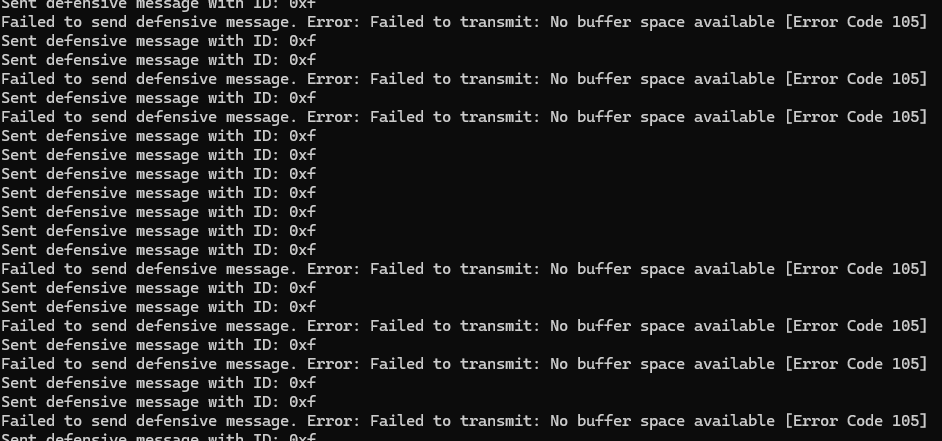
\includegraphics[width=0.9\linewidth]{buffer_full.png}
    \caption{Buffer error on the software side}
    \label{fig:lost_messages}
\end{figure}
\begin{figure}
    \centering
    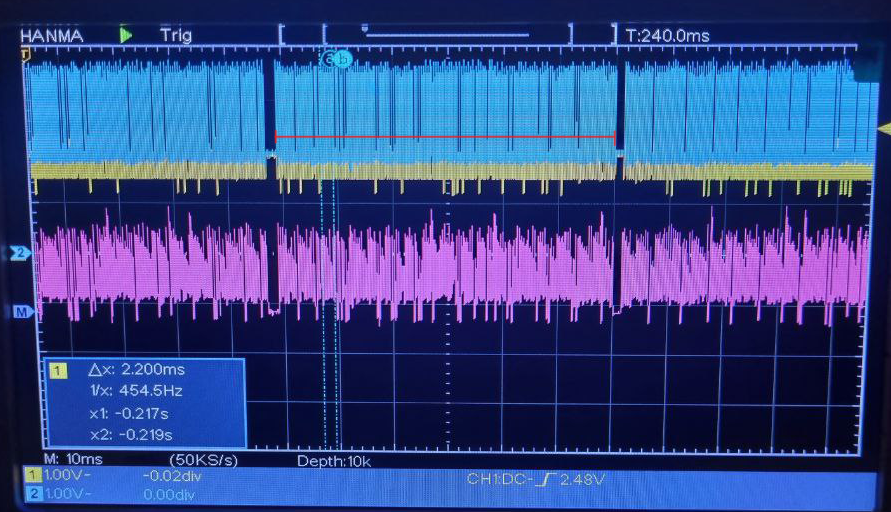
\includegraphics[width=0.9\linewidth]{scope.png}
    \caption{Holes on the CAN bus signal due to buffer error}
    \label{fig:scope}
\end{figure}

As a second attempt, the attacker rate was reduced to 0.25 seconds, in that way the defender should send only $250/(0.210 + 0.180) = 641$ messages to reach the start of the next spoofed message.
The 642th message should trigger the first step of the defense mechanism, forcing the attacker into a bus-off state without overloading the CAN controller buffer.
The experiment was unsuccessful, as we were still getting the same buffer error as before.


\section{Conclusion}

The experiment demonstrated the challenges of implementing the Parrot system on low-end, cost-effective devices.
According to the MCP2515 datasheet, the CAN controller should be able to transmit messages up to 1~Mbps, but in the experiment, the actual bitrate was limited to 
500~Kbps. This discrepancy arose from the fact that the purchased CAN shields used an 8~MHz crystal oscillator instead of the specified 16~MHz one.
Without the ability to transmit messages at a very high rate, the Parrot system cannot disarm the attacker, making it ineffective in a real-world scenario.
The authors of the original paper stated that the CAN controller should be able to send one message every 31~$\mu$s to effectively disarm the attacker, but in the experiment, the actual rate achieved was one message every 390~$\mu$s.



{\small
    \bibliographystyle{ieee_fullname}
    \bibliography{paper}
}

\end{document}